\documentclass{article}
\usepackage{amsmath}
\usepackage{amssymb}
\usepackage{algorithm}
\usepackage{float}
\usepackage{color}
\usepackage{multicol}
\usepackage{forloop}
\usepackage{graphicx}
\usepackage[margin=0.8in]{geometry}
\usepackage{caption}
\usepackage{enumerate}

\graphicspath{ {.} }
\title{MATH 3800 F\\
	\large{Assignment 2}}
\author{Krystian Wojcicki, 101001444}
\date{Winter 2020}

\begin{document}
\maketitle

\begin{enumerate}[1.]

\item \textbf{Use Least-Squares to fit a straight line, $y = ax + b$, to the data. Plot the data and the
line. Caclulate R2 and comment on the quality of the fit. \\
\begin{tabular}{ c | c c c c c c}
x              & 1 & 3 & 4 & 7 & 10  & 12 \\
\hline
y & 2.16 & 9.42 & 13.05 & 23.77 & 34.58 & 41.83  \\
\end{tabular}} 

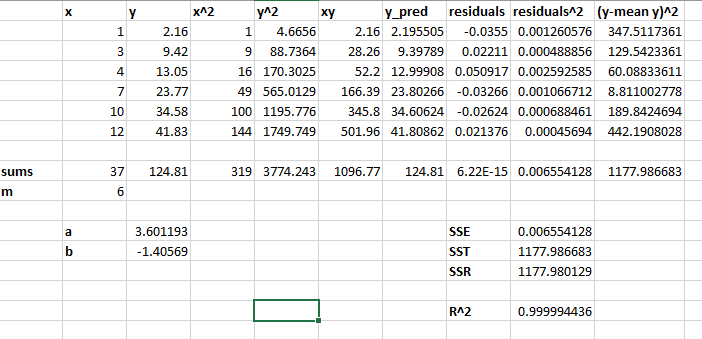
\includegraphics[width= 0.95\textwidth]{a2_q1_data} \\
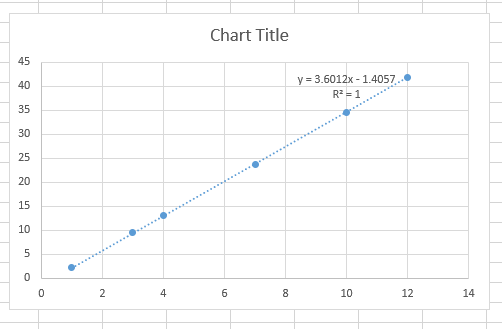
\includegraphics{a2_q1_graph} \\
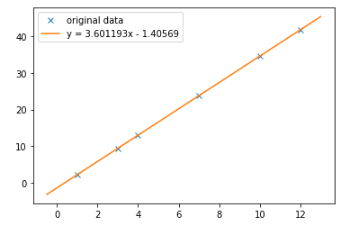
\includegraphics{a2_q1_python}

As we can see from the value of $R^2$ and the plot of the data, the fit is excellent.

\item \textbf{Use Least-Squares to fit a curve, $y = ae^{bx}$, to the appropriate transformation of the data.
Plot the data and the curve. Caclulate $R^2$ and comment on the quality of the fit. \\
\begin{tabular}{ c | c c c c c c}
x              & 0.5 & 1 & 1.7 & 2.2 & 3  & 3.6 \\
\hline
y & 0.425 & 0.605 & 0.987 & 1.400 & 2.448 & 3.728  \\
\end{tabular}}

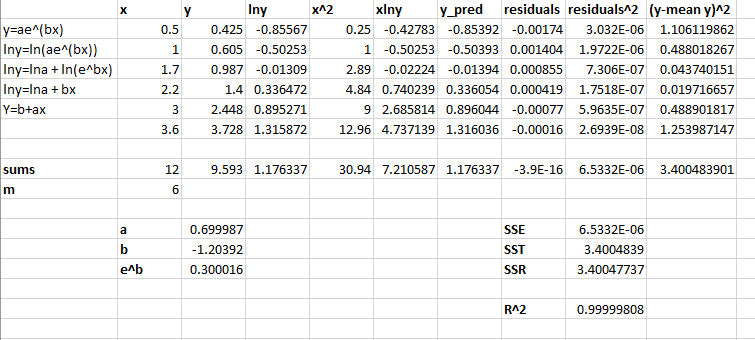
\includegraphics[width= 0.95\textwidth]{a2_q2_data} \\
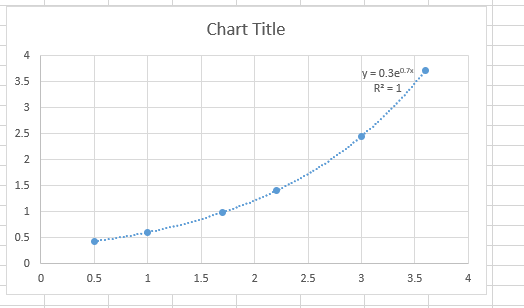
\includegraphics{a2_q2_graph} \\
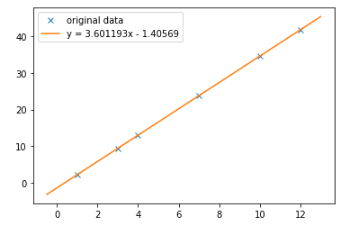
\includegraphics{a2_q1_python}

The $R^2$ on the transformed/linear data is excellent  and once again the fit is excellent.

\item \textbf{
Use the Ladder of Powers Transformations to determine if a simple/one-term model
would be an appropriate fit. Which functional form seems best ? (You do not have to fit the
curve.) \\
\begin{tabular}{ c | c c c c c c c c c c }
x              & 1 & 2 & 3 & 4 & 5  & 6 & 7 & 8 & 9 & 10 \\
\hline
y & 0 & 4.27 & 6.82 & 8.60 & 10 & 11.13 & 12.04 & 12.88 & 13.61 & 14.25  \\
\end{tabular}}

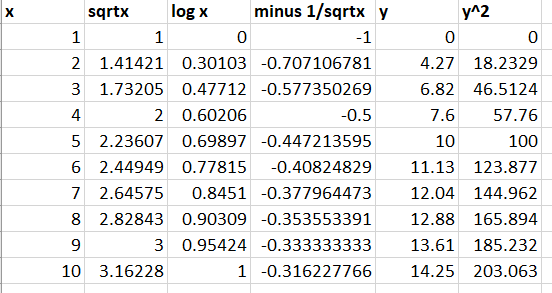
\includegraphics[width= 0.95\textwidth]{a2_q3_data} \\
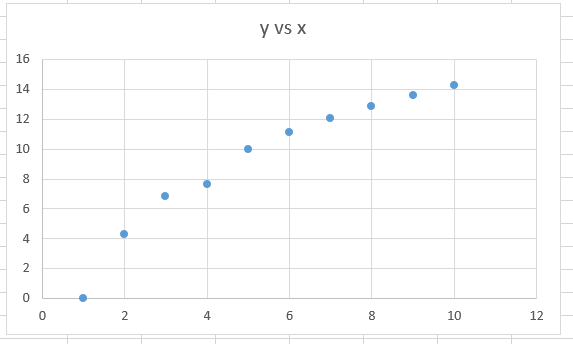
\includegraphics{a2_q3_org} \\

Data is increasing and concave down, so we will try $x \Rightarrow \sqrt{x}, log(x), ...$ on $y \Rightarrow y, y^2$

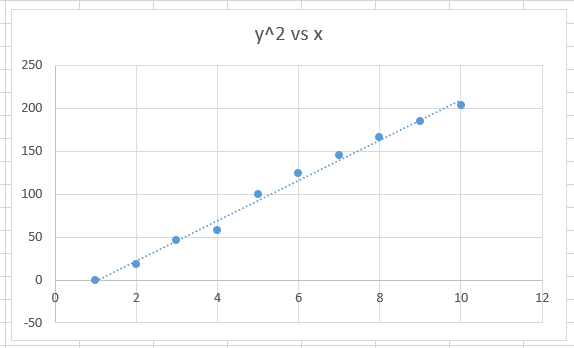
\includegraphics{a2_q3_graph1} \\
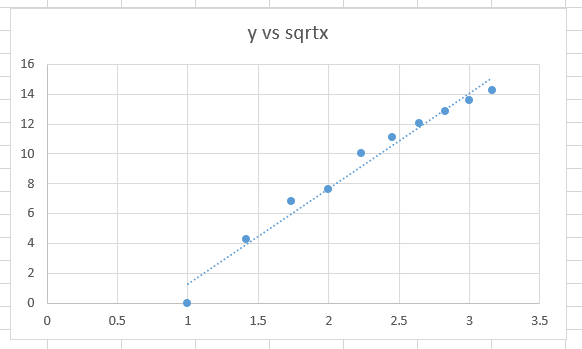
\includegraphics{a2_q3_graph2} \\
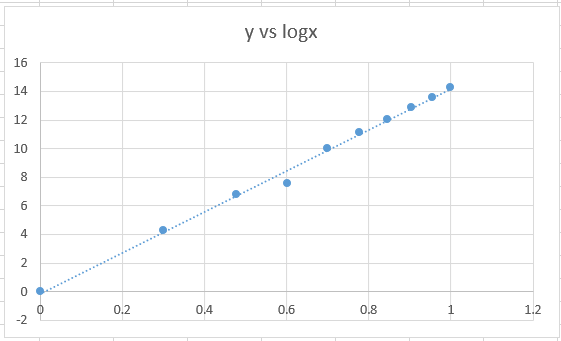
\includegraphics{a2_q3_graph3} \\
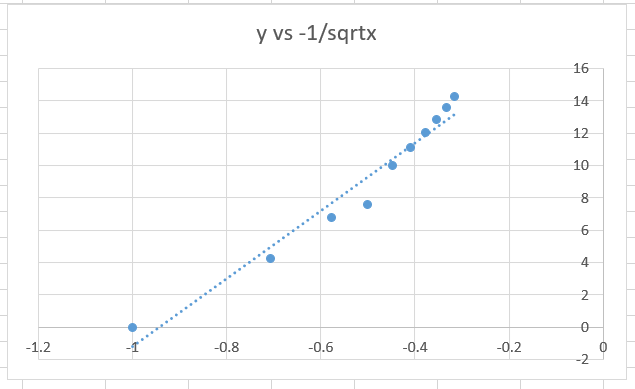
\includegraphics{a2_q3_graph4}


\item \textbf{Consider the data below. Construct a divided difference table and determine if a
low-order polynomial would be appropriate as an empirical model. \\
\begin{tabular}{ c | c c c c c c c c }
x              & 0 & 1 & 2 & 3 & 4 & 5  & 6 & 7 \\
\hline
y & 1 & 4.5 & 20 & 90 & 403 & 1808 & 8103 & 36316 \\
\end{tabular}}

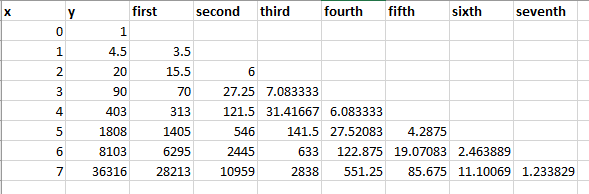
\includegraphics{a2_q4}

From the divided difference table we can see that there is no column that is relatively constant (or relatively close to 0). So we can conclude that a low order polynomial would not be appropriate for this data.

\item \textbf{ Find the natural cubic spline for the points (0, 0),(2, 5) and (4, 7).}

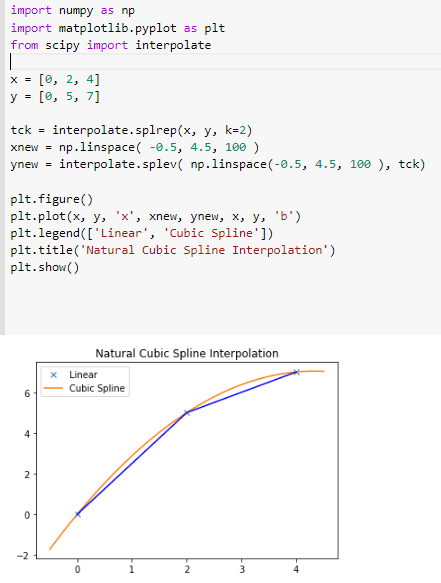
\includegraphics{a2_q5} \\

\begin{gather} \label{eq:1}
y_1 = S_1(x_1) : 0 = a_1 \\
y_2 = S_1(x_2) : 5 = a_1 + 2b_1 + 4c_1 + 8d_1 \\
y_2 = S_2(x_2) : 5 = a_2 + 2b_2 + 4c_2 + 8d_2 \\
y_3 = S_2(x_3) : 7 = a_2 + 4b_2 + 16c_2 + 64d_2 \\
S_1\prime(x) = b_1 + 2xc_1 + 3x^2d_1 \nonumber \\
S_2\prime(x) = b_2 + 2xc_2 + 3x^2d_2 \nonumber \\
S_1\prime\prime(x) = 2c_1 + 6xd_1 \nonumber \\
S_2\prime\prime(x) = 2c_2 + 6xd_2 \nonumber \\
S_1\prime(x_2)  = S_2\prime(x_2):  b_1 + 4c_1 + 12d_1 = b_2 + 4c_2 + 12d_2\\
S_1\prime\prime(x_2) = S_2\prime\prime(x_2) : 2c_1 + 12d_1 = 2c_2 + 12d_2\\
S_1\prime\prime(x_1) = 0 : 2c_1 + 0 = 0 \\
S_2\prime\prime(x_3) = 0 : 2c_2 + 24d_2 = 0
\end{gather}

From (1) $\Rightarrow a_1 = 0$ \\
From (7) $\Rightarrow c_1 = 0$ \\
Substitute $c_1 = 0$ into (6) $\Rightarrow 12d_1 = 2c_2 + 12d_2 \Rightarrow d_1 = -d_2$ and $c_2 = -12d_2$\\
Substitute $c_1 = 0, d_1 = -d_2$ into (5) $\Rightarrow b_1 + 12d_1 = b_2 + 4c_2 + 12d_2 \Rightarrow b_1 - b_2 = -24d_2 \Rightarrow b_1 = b_2 - 24d_2, b_2 = b_1 + 24d_2$ \\
Substitute $a_1 = 0, c_1 = 0, b_1 = b_2 - 24d_2, d_1 = -d_2$ into (2) and (3) $\Rightarrow 2b_2 - 48d_2 - 8d_2 = a_2 + 2b_2 - 40d_2 \Rightarrow a_2 = -16d_2$ \\
Substittue $a_2 = -16d_2, c_2 = -12d_2$ into (4) $\Rightarrow 7 = -16d_2 + 4b_2 + 16(-12d_2) + 64d_2 \Rightarrow b_2 = \frac{7}{4} + 36d_2$ \\
Substitute $b_2 = \frac{7}{4} + 36d_2$ into $b_2 = b_1 + 24d_2 \Rightarrow \frac{20}{7}(b_1 - 12d_2) = 5$ \\
Substitute $ \frac{20}{7}(b_1 - 12d_2) = 5, a_1 = 0, c_1 = 0, d_1 = -d_2$ into (2) $\Rightarrow \frac{20}{7}b_1 - \frac{240}{7}d_2 = 2b_1 - 8d_2 \Rightarrow b_1 = \frac{92}{3}d_2$ \\
Substitute $b_1 = 92/3d_2$ into $b_1 - 12d_2 = \frac{7}{4} \Rightarrow d_2 = \frac{3}{32}$ \\

Therefore $a_1 = 0, b_1 = (92/3) * (3/32) = \frac{23}{8}, c_1 = 0, d_1 = -\frac{3}{32}, a_2 = -16 * (3/32) = -1.5, b_2 = \frac{23}{8} + 24 * (3/32) = \frac{41}{8}, c_2 = -12 * \frac{3}{32} = -\frac{9}{8}, d_2 = \frac{3}{32}$

Giving us
$\begin{cases} 
S_1(x) = \frac{23}{8}x - \frac{3}{32}x^3, 0 \leq x \leq 2 & \\
S_2(x) = -1.5 + \frac{41}{8}x - \frac{9}{8}x^2 + \frac{3}{32}x^3, 2 \leq x \leq 4
\end{cases}
$

Check to ensure that given points are in the cubic spine function created. And indeed $S_1(0) = 0, S_1(2) = 5, S_2(2) = 5, S_2(4) = 7$.

\end{enumerate}
\end{document}